\begin{center}
\begin{tikzpicture}[scale=0.9, transform shape]

\node[inner sep=0pt] (russell) at (0,0)
    {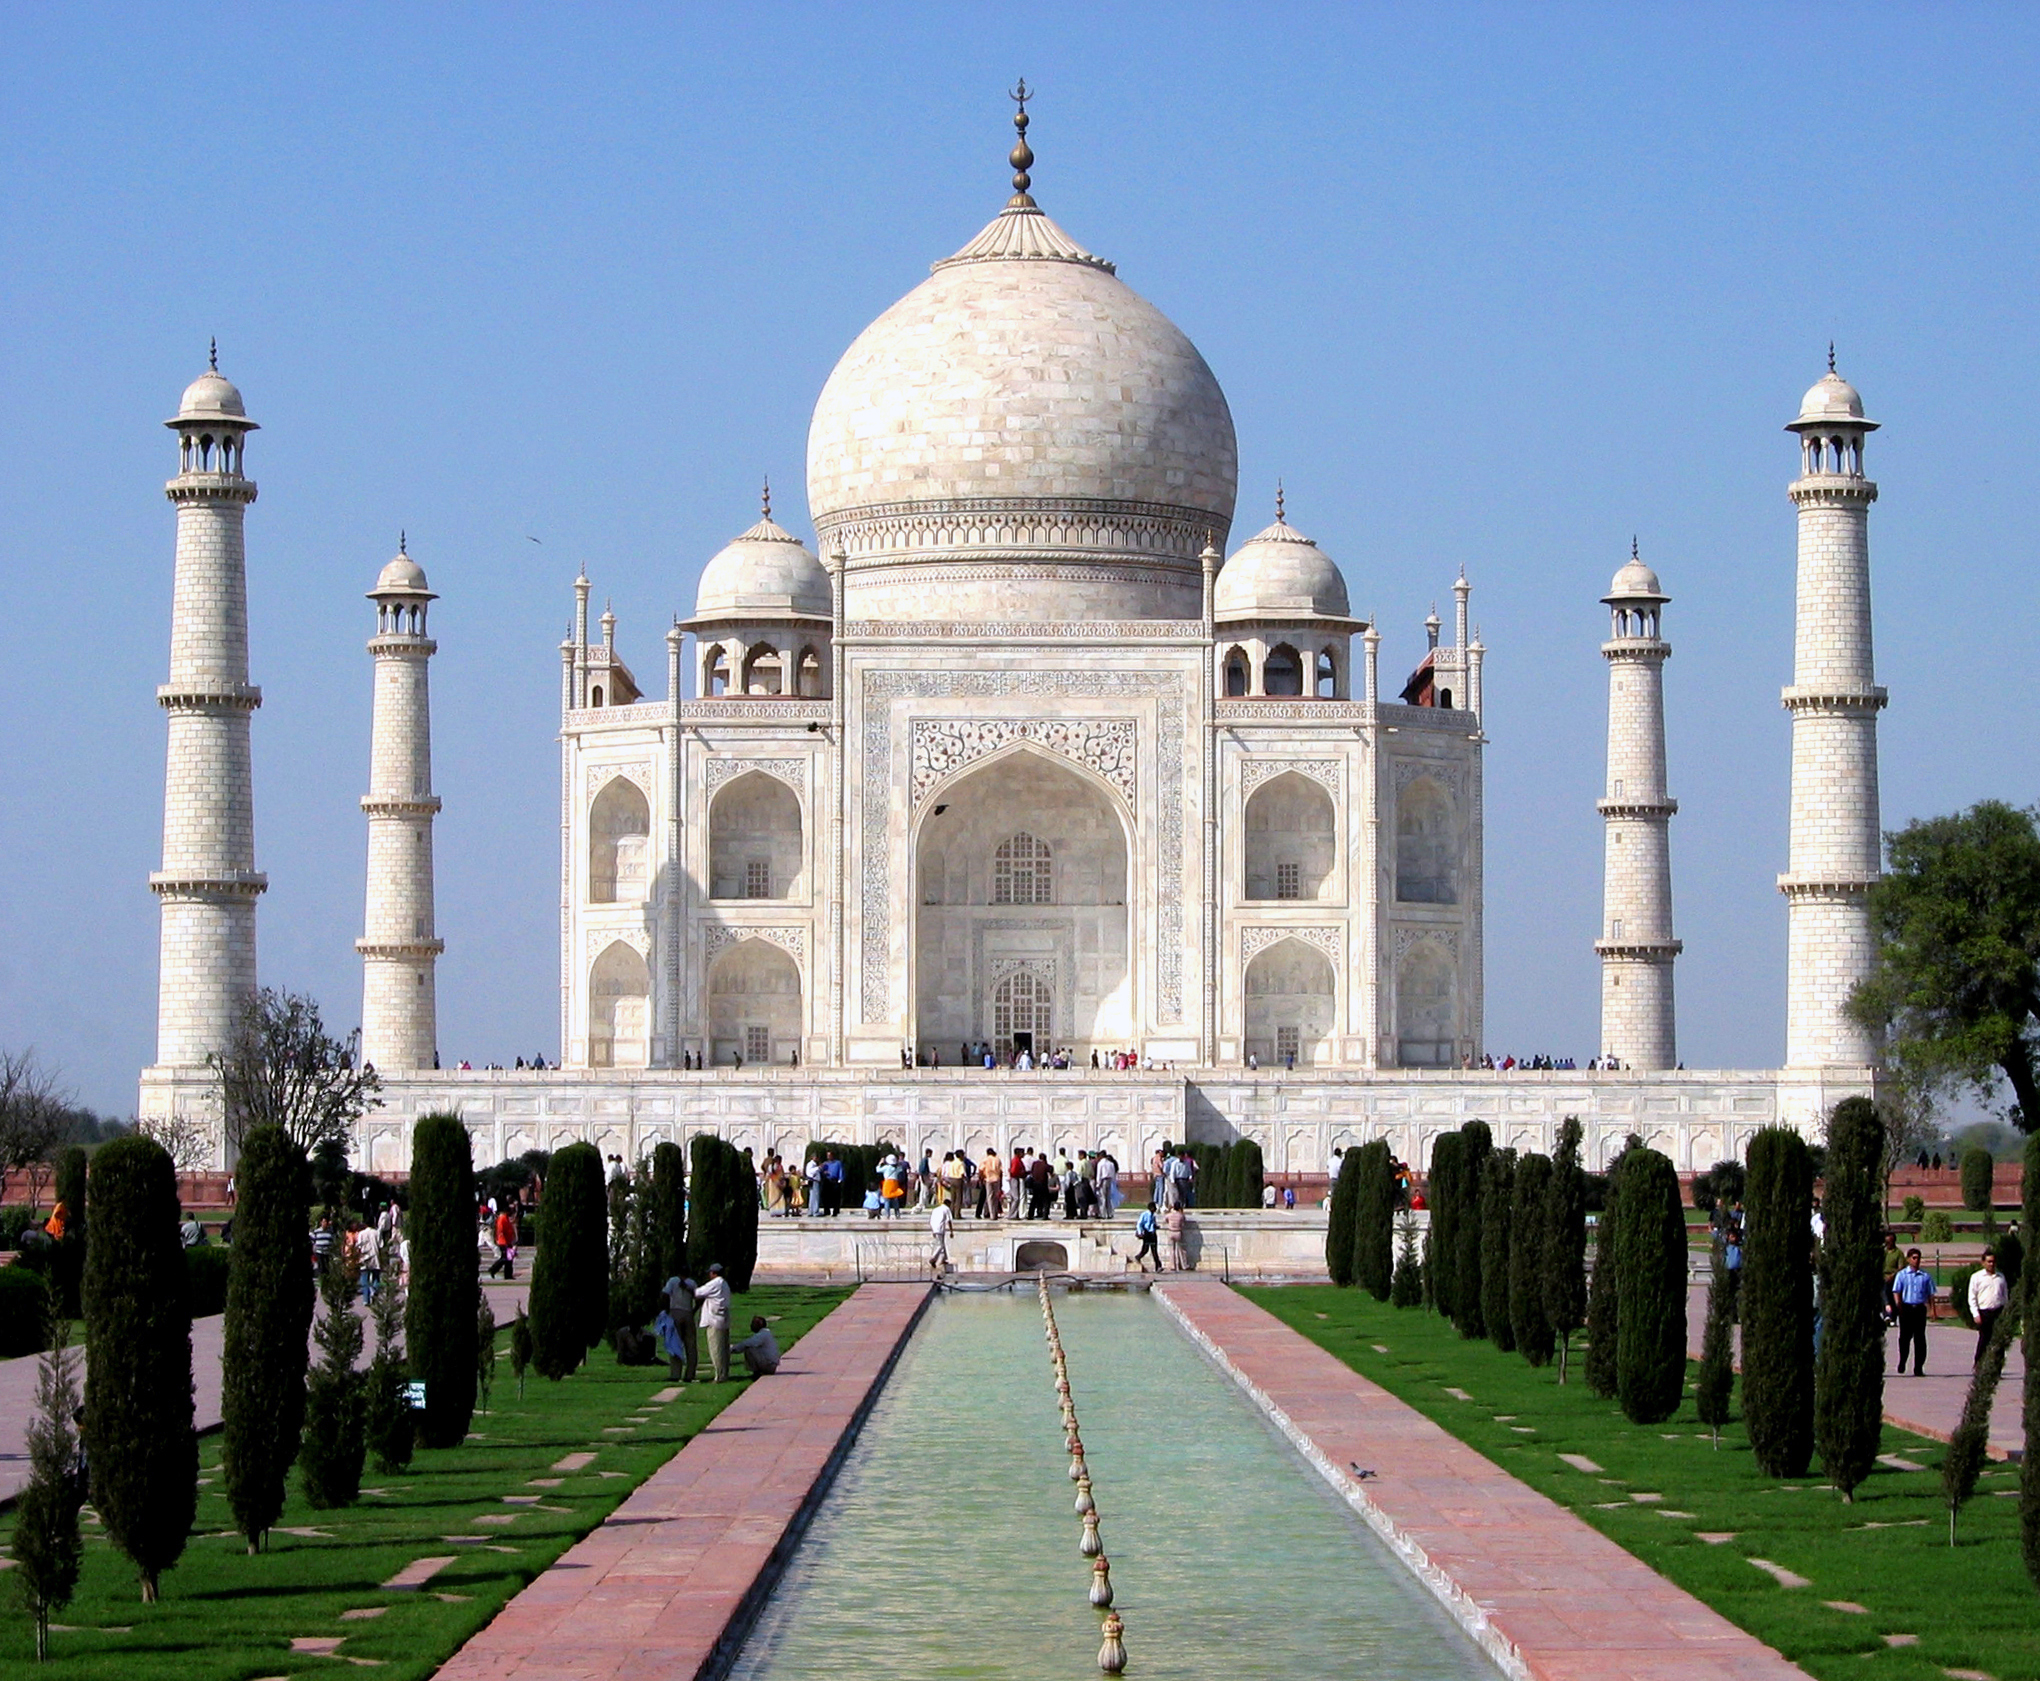
\includegraphics[origin=rt, angle=5, width=0.5\linewidth,height=\linewidth]{images/tajmahal.jpg}};

\def\x{0.3}
\def\y{0.33}
%drawing lines
\foreach \mv in {0,...,11}
	\draw (-1.76+\x*\mv,-1.76*0.23+3.5+\x*\mv*0.23) -- (-1.55+\x*\mv,-1.55*0.23-3.5+\x*\mv*0.23);

\foreach \mv in {0,...,21}
	\draw (-\y*\mv*-0.035+3.86*-0.035+1.66,+3.86-\y*\mv) -- (-\y*\mv*-0.035+3.1*-0.035-1.66,3.1-\y*\mv);

\def\xa{-1.7685}
\def\ya{3.1}
\def\swx{0.2994}
\def\swy{0.0658}
\def\shx{0.0116}
\def\shy{0.33}
\def\xw{0.8982}
\def\yw{0.197}
\def\xh{0.035}
\def\yh{-0.99}

\foreach \my [count=\yi from 0] in {0,...,18}{
	\foreach \mx [count=\xi from \yi*9+2] in {0,...,8}{
	\ifthenelse{\xi<8}{
	\onslide<\xi>{
		\edef\xla{\xa+\mx*\swx+\my*\shx}				
		\edef\yla{\ya+\mx*\swy-\my*\shy}
		%\xdef\xa{\xa+\mx*\swx+\my*\shx}
		%\xdef\ya{\ya+\mx*\swy-\my*\shy}
		\draw[black,line width=1.5pt] (\xla,\yla) -- (\xla+\xw,\yla+\yw) -- (\xla+\xw+\xh,\yla+\yw+\yh) -- (\xla+\xh,\yla+\yh) -- cycle;	

		\edef\xta{4+\xla+\xw*0.5+\xh*0.5}		
		\edef\yta{\yla+\yw*0.5+\yh*0.5+0.05}
		\draw[black!50] (\xla,\yla) -- (\xta,\yta) (\xla+\xw,\yla+\yw) -- (\xta,\yta)  (\xla+\xw+\xh,\yla+\yw+\yh) -- (\xta,\yta) (\xla+\xh,\yla+\yh) -- (\xta,\yta);
		}
	\onslide<\xi->{
		\fill (\xta,\yta) circle (2pt);
		}	
	}{
	\ifthenelse{\xi > 7 \AND \xi < 160}{
	\onslide<8->{
		\edef\xla{\xa+\mx*\swx+\my*\shx}				
		\edef\yla{\ya+\mx*\swy-\my*\shy}
		%\xdef\xa{\xa+\mx*\swx+\my*\shx}
		%\xdef\ya{\ya+\mx*\swy-\my*\shy}
		\edef\xta{4+\xla+\xw*0.5+\xh*0.5}		
		\edef\yta{\yla+\yw*0.5+\yh*0.5+0.05}
	
		\fill (\xta,\yta) circle (2pt);
		}
	}{
	 \pgfmathparse{int(\xi-160+8)}
	 \onslide<\pgfmathresult>{
		\edef\xla{\xa+\mx*\swx+\my*\shx}				
		\edef\yla{\ya+\mx*\swy-\my*\shy}
		%\xdef\xa{\xa+\mx*\swx+\my*\shx}
		%\xdef\ya{\ya+\mx*\swy-\my*\shy}
		\draw[black,line width=1.5pt] (\xla,\yla) -- (\xla+\xw,\yla+\yw) -- (\xla+\xw+\xh,\yla+\yw+\yh) -- (\xla+\xh,\yla+\yh) -- cycle;	

		\edef\xta{4+\xla+\xw*0.5+\xh*0.5}		
		\edef\yta{\yla+\yw*0.5+\yh*0.5+0.05}
		\draw[black!50] (\xla,\yla) -- (\xta,\yta) (\xla+\xw,\yla+\yw) -- (\xta,\yta)  (\xla+\xw+\xh,\yla+\yw+\yh) -- (\xta,\yta) (\xla+\xh,\yla+\yh) -- (\xta,\yta);
		}
	\onslide<\pgfmathresult->{
		\fill (\xta,\yta) circle (2pt);
		}
	
	};
	};
			
	}
}

\onslide<2->{
\foreach \mv in {1,...,10}
	\draw (4-1.76+\x*\mv,-1.76*0.23+3.5+\x*\mv*0.23+\swy-\shy) -- (4-1.55+\x*\mv,-1.55*0.23-3.5+\x*\mv*0.23+\swy+\shy);

\foreach \mv in {1,...,20}
	\draw (4-\y*\mv*-0.035+3.86*-0.035+1.66-\swx+\shx,+3.86-\y*\mv) -- (4-\y*\mv*-0.035+3.1*-0.035-1.66+\swx+\shx,3.2-\y*\mv);
}


\end{tikzpicture}
\end{center}